\section{Antal}
\setbeamertemplate{caption}{\raggedright\insertcaption\par}
\begin{frame}{Introduction}{Antal János Monori\newline<amonor14@student.aau.dk>}
	\begin{figure}[h!]
		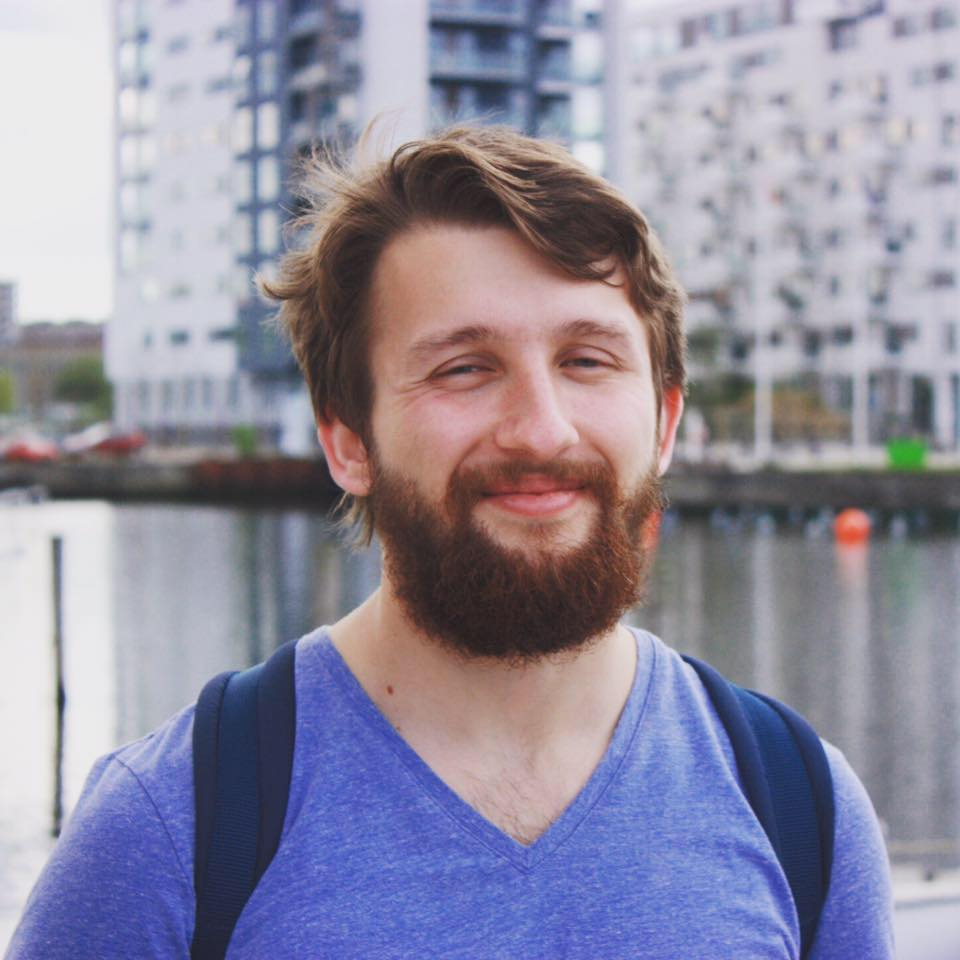
\includegraphics[width=0.3\textwidth]{images/anthony.jpg}
		\caption{Antal János Monori}
		\centering    		
	\end{figure}
\end{frame}

\setbeamertemplate{caption}[default]

\begin{frame}{Overview}{Antal János Monori\newline<amonor14@student.aau.dk>}
	Presentation Agenda
	\begin{itemize}
		\item Introduction
		\item Testing and Prototyping
		\item Future steps
		\item Process analysis
	\end{itemize}
\end{frame}


\begin{frame}{Introduction}{Antal János Monori\newline<amonor14@student.aau.dk>}
	\begin{itemize}
		\item <2-> Mapping and Navigation of unknown terrain
		% Let's decode the title a bit and look at the individual parts a bit more in depth
		\begin{itemize}
			\item <3-> Mapping % idea behind, motivation, problem to solve
			\item <4-> Navigation % idea behind, motivation, problem to solve
			\item <5-> Unknown terrain % idea behind, motivation, problem to solve
		\end{itemize}
		\item <6-> 3D mapping, full autonomous navigation, etc. % what we have in plans for the future development of the idea (short-motivation)
	\end{itemize}
\end{frame}

\begin{frame}{Approach}{Antal János Monori\newline<amonor14@student.aau.dk>}
	\begin{itemize}
		\item <2-> 1. Idea came from common interest
		\item <3-> 2. Preliminary research
		\item <4-> 3. Focused prototype and scope
		\item <5-> 4. Stakeholder and risk analysis
	\end{itemize}
\end{frame}

\begin{frame}{Scope}{Antal János Monori\newline<amonor14@student.aau.dk>}
	To make a rover capable of 2D mapping of unknown terrains and finding its own path to navigate across it, then providing a usable 2D map of the surroundings from point A to B.
\end{frame}

\begin{frame}{Prototype}{Antal János Monori\newline<amonor14@student.aau.dk>}
	\begin{figure}[h!]
		\only<1>{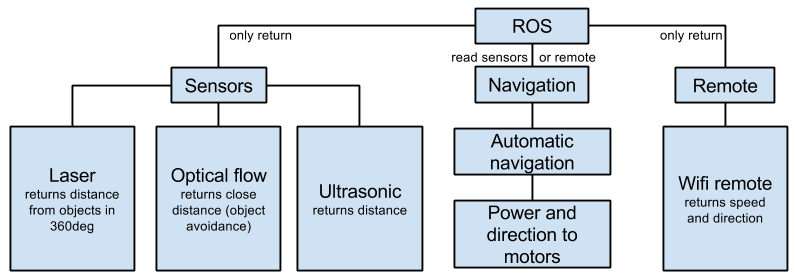
\includegraphics[width=0.9\textwidth]{images/developmentdiagram.png}}
		\only<2>{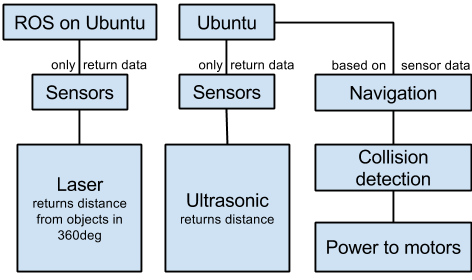
\includegraphics[width=0.7\textwidth]{images/developmentdiagram2.png}}
	\end{figure}
\end{frame}

\begin{frame}{Prototype}{Antal János Monori\newline<amonor14@student.aau.dk>}
	\begin{itemize}
		\item We split up the prototype into two parts:
		\begin{itemize}
			\item <2-> Navigation-module
			\item <3-> Mapping-module
		\end{itemize}
		\item <4-> Motivation behind this:
		\begin{itemize}
			\item <5-> Individual development
			\item <6-> Decoupling -> avoid risks and unnecessary dependencies
		\end{itemize}
	\end{itemize}
\end{frame}

\begin{frame}{Components - Navigation module}{Antal János Monori\newline<amonor14@student.aau.dk>}
	\begin{itemize}
		\item - HC-SR04 Ultrasonic Range Finder (3 of them)
		\item - DFRobot 4WD Arduino-Compatible Platform with Encoders
		\item - Pololu DRV8833		
		\item - Raspberry Pi 2 Model B ARM Cortex-A7 Quad Core CPU 900MHz 1GB RAM 
		\item - CJMCU-110 Optical Flow Sensor w/ Pin Header for APM2.52/ APM2.6 - Purple	(not used afterall)
		\item - 3D printed enclosures for ultrasonic sensors
	\end{itemize}
\end{frame}

\begin{frame}{But how does it actually work?}{Antal János Monori\newline<amonor14@student.aau.dk>}
	%\begin{itemize}
	%	\item 
	%\end{itemize}
	\begin{figure}[h!]
		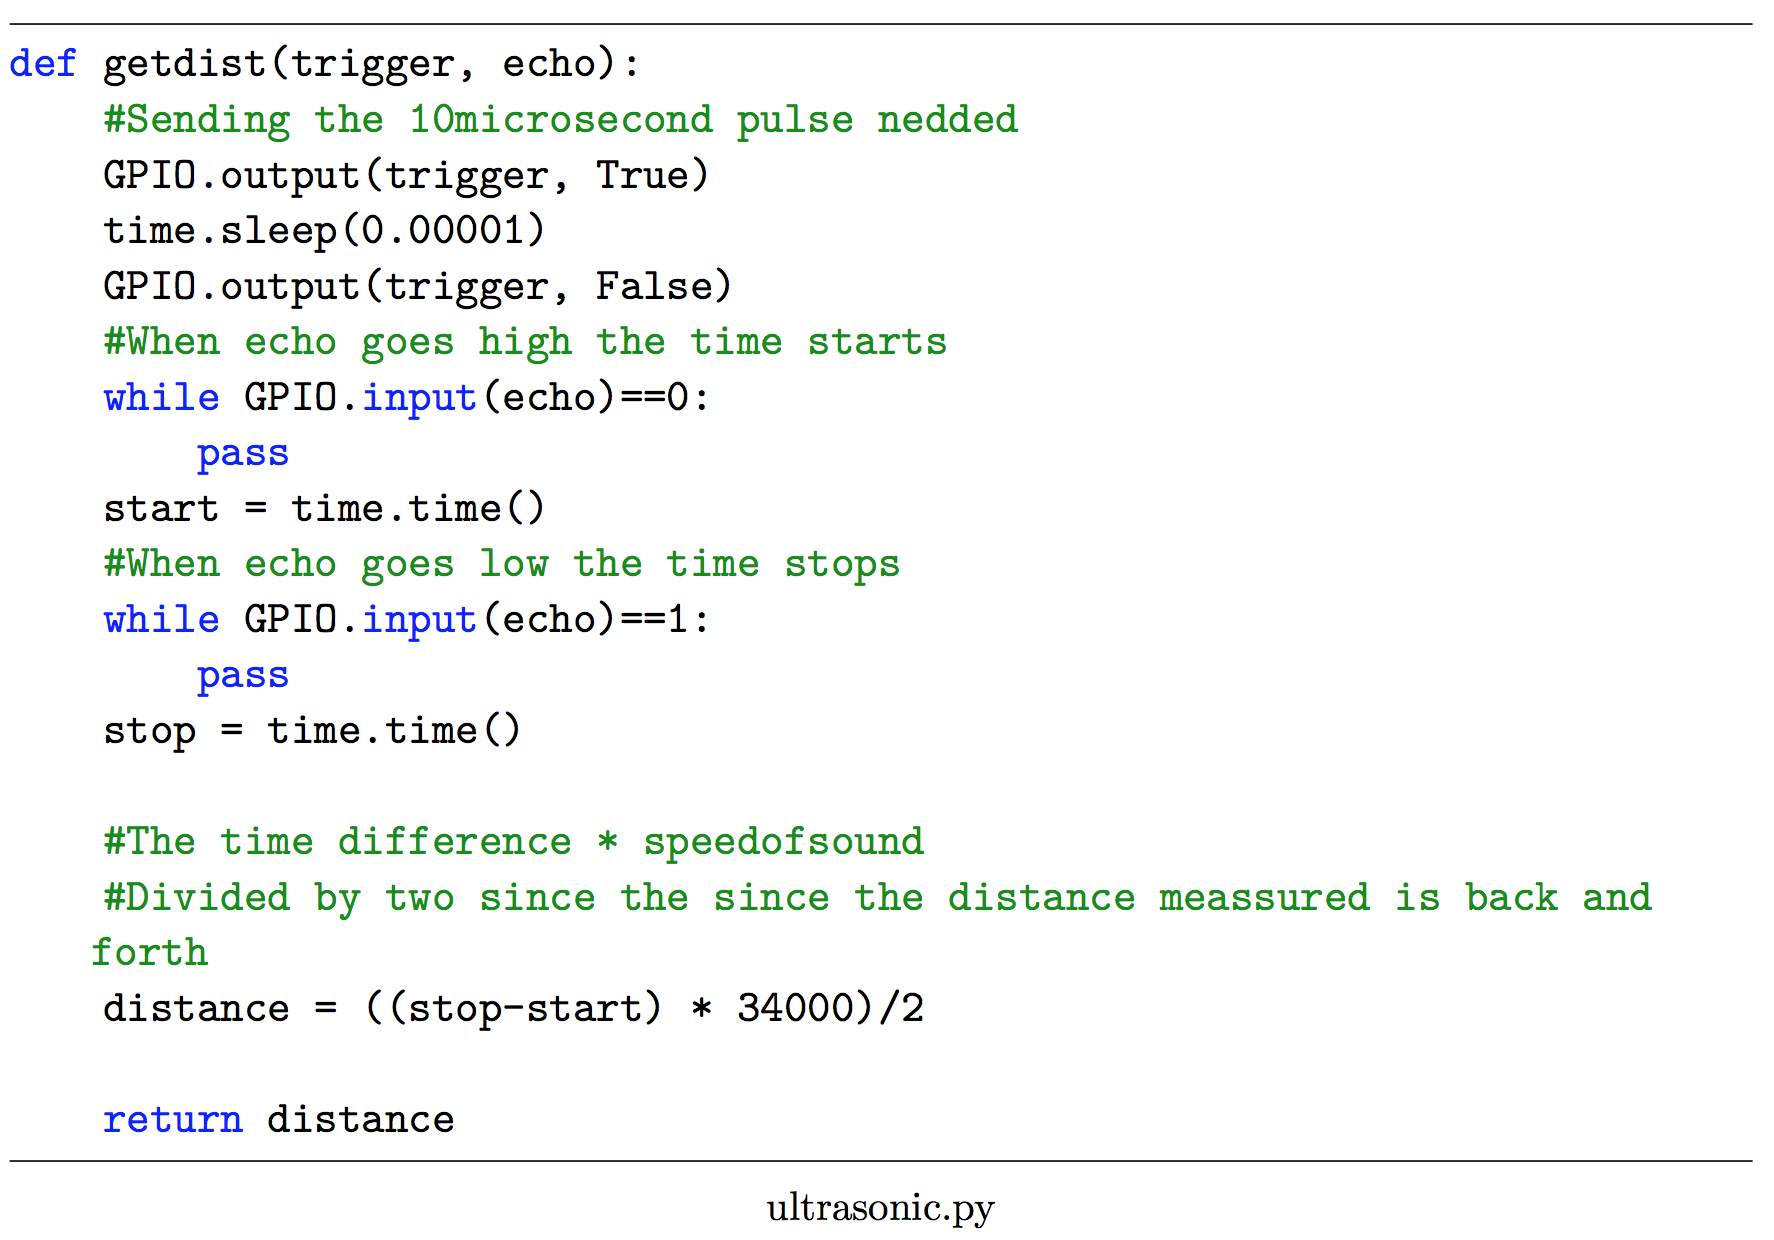
\includegraphics[width=0.9\textwidth]{images/dissensor.png}
	\end{figure}
\end{frame}

\begin{frame}{But how does it actually work?}{Antal János Monori\newline<amonor14@student.aau.dk>}
	%\begin{itemize}
	%	\item 
	%\end{itemize}
	\begin{figure}[h!]
		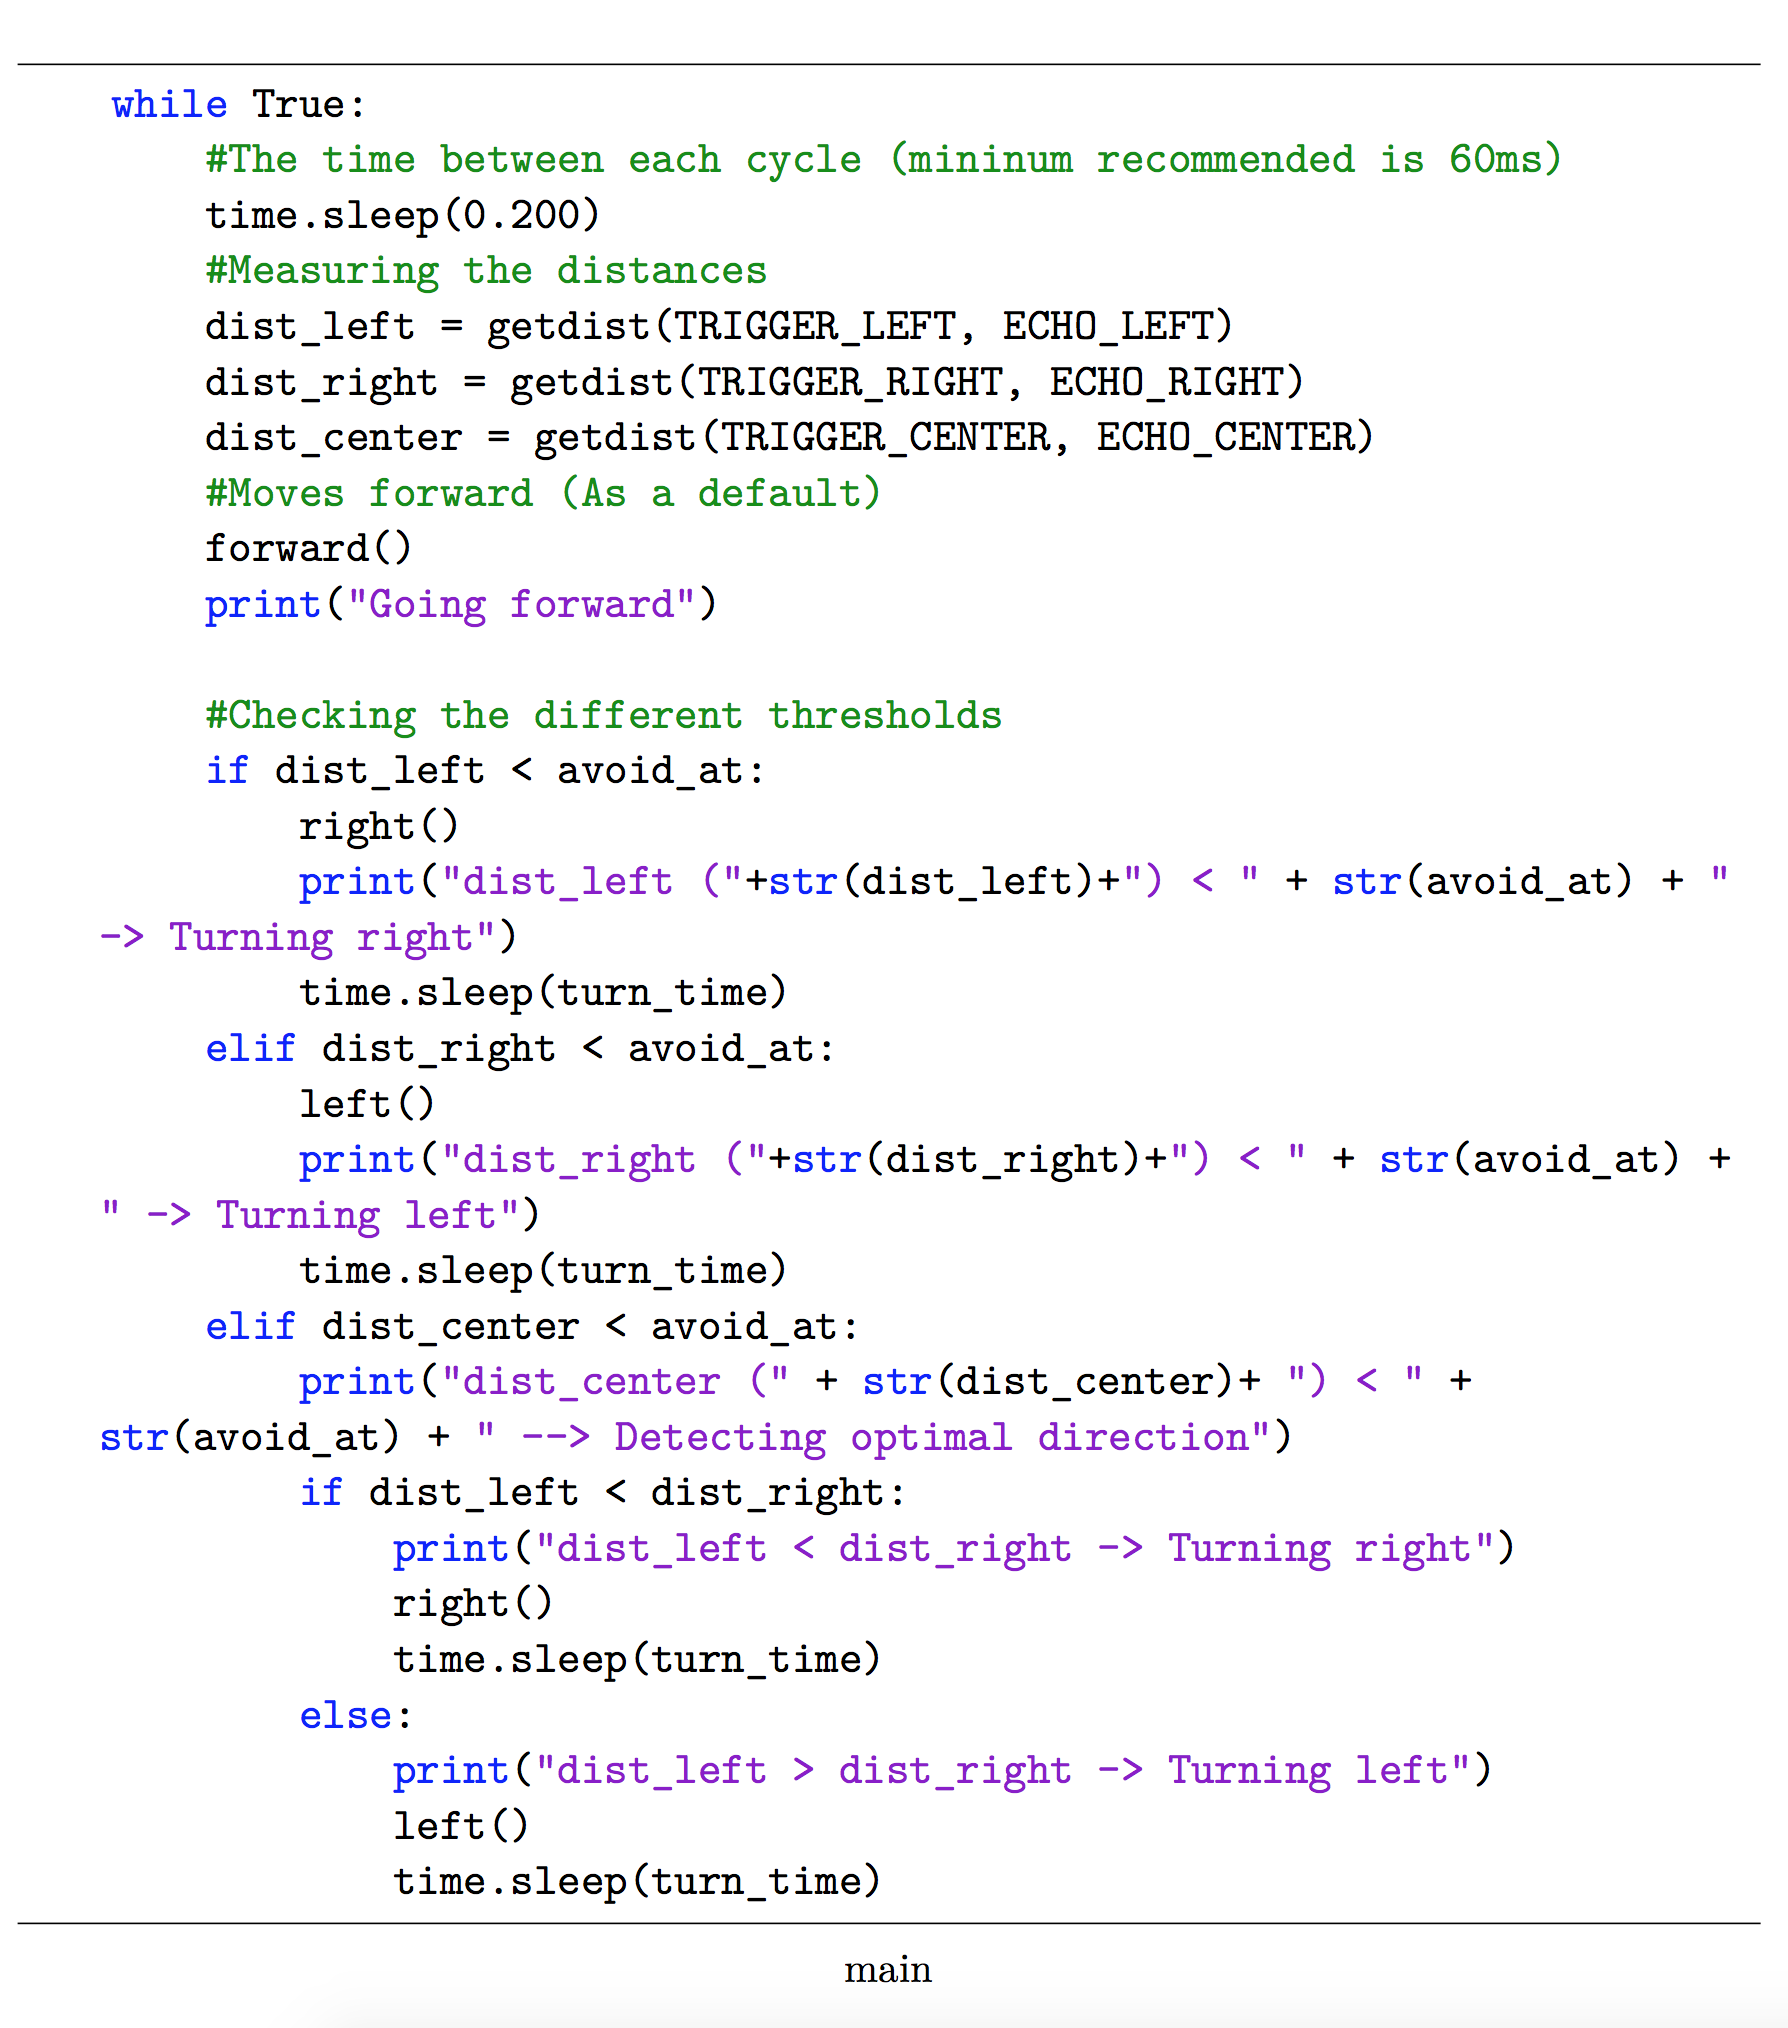
\includegraphics[width=0.7\textwidth]{images/navcode.png}
	\end{figure}
\end{frame}

\begin{frame}{Components - Mapping module}{Antal János Monori\newline<amonor14@student.aau.dk>}
	\begin{itemize}
		\item - LIDAR-Lite Laser Rangefinder
		\item - Slip Ring with 22mm rim
		\item - 12V, 350mA, 28oz-in NEMA-17 Bipolar Stepper Motor
		\item - EasyDriver - Stepper Motor Driver
		\item - 3D printed case for microcontroller and stepper motor
		\item - Raspberry Pi 2 Model B ARM Cortex-A7 Quad Core CPU 900MHz 1GB RAM 
		\item - Arduino Mega 2560
	\end{itemize}
\end{frame}